\documentclass[12pt, letterpaper]{article}
\usepackage[utf8]{inputenc}

\usepackage[margin=1in]{geometry}
\usepackage{mathpazo}

\usepackage{graphicx}
\usepackage{amsmath}
\title{Stochastic Conditional Layers: Embodiments, Architecture, Training and Inference}
\date{}

\usepackage[font={small,sf,bf}]{caption}

\begin{document}
\vspace{-5cm}
\maketitle
\vspace{-2cm}
Stochastic conditional layers are trainable parameters used to define a noise distribution, where the parameters depend on labels or categories present in the training dataset. The stochastic conditional layers are combined using selection layers for the task of inference, when the labels or categories of the inputs remain unknown. The stochastic conditional layers are used to obfuscate a given input, such that the inference accuracy is not compromised.  

\section{Architecture}
We categorize the stochastic conditional layers based on their architecture.
Any trainable network or layer(s) with trainable parameters can act as stochastic conditional layers. 
These include (but are not limited to) additive layers, convolutional layers, fully connected layers, recurrent layers like Long Short Term Memory (LSTM), Gated Recurrent Unit (GRU), transformer layers, etc. In this section we discuss stochastic conditional convolutional layers and  stochastic conditional fully connected layers as physical incarnations of the stochastic conditional layers. 

\subsection{Stochastic Conditional Convolutional Layers}
We discuss stochastic conditional convolutional layers (Sec.~\ref{sec:stochasticcondconv}) by first laying the ground for convolutional layers (Sec.~\ref{sec:conv}) and conditional convolutional layers (Sec.~\ref{sec:condconv}).

\subsubsection{Convolutional Layers}
\label{sec:conv}
Convolution (in the context of neural networks) is a linear mathematical operation where a kernel $k$ slides across an input tensor $x$ performing a linear operation at every location of the tensor $x$, thereby transforming $x$ in a certain way. 
The output of this operation is a tensor $h_k$ which represents a feature (also called an activation). 
In a convolutional layer of a neural network, the input tensor $x$ is passed through a number of parameterized kernels, whose parameters are learnt during training through backpropagation. 
The activations $h_k$ from the respective kernels $k$ are stacked into channels to form the output $h=[h_k]$. Eq.~\eqref{eq:conv} shows the convolution operation. 
In Eq.~\eqref{eq:conv}, $[m,n]$ represents the spatial coordinates of the output tensor $h_k$, $[i,j]$ represents the spatial coordinates of the kernel $k$.
\begin{equation}
  h_k[m,n]=(x * k)[m,n]=\sum_i \sum_j k[i,j]x[m+i,n+j]
  \label{eq:conv}
\end{equation}

\subsubsection{Conditional Convolutional Layers}
\label{sec:condconv}
Deep networks are often employed for tasks that involve categorizing objects into a specific category from the training dataset. For example, object classification involves determining whether a given image is of a cat or a dog. Object detection involves the same, with the additional task of localizing the animal spatially. It can be useful to learn convolutional kernels specific to the category of objects. In other words, convolutional layers can be conditioned on the category of object. This is shown in Eq.~\eqref{eq:condconv}, where $k_c$ represents the kernels specific to the category $c$ in the training dataset.

\begin{equation}
  h_{k_c}[m,n]=(x * k_c)[m,n]=\sum_i \sum_j k_c[i,j]x[m+i,n+j]
  \label{eq:condconv}
\end{equation}
\begin{figure}[t]
    \centering
    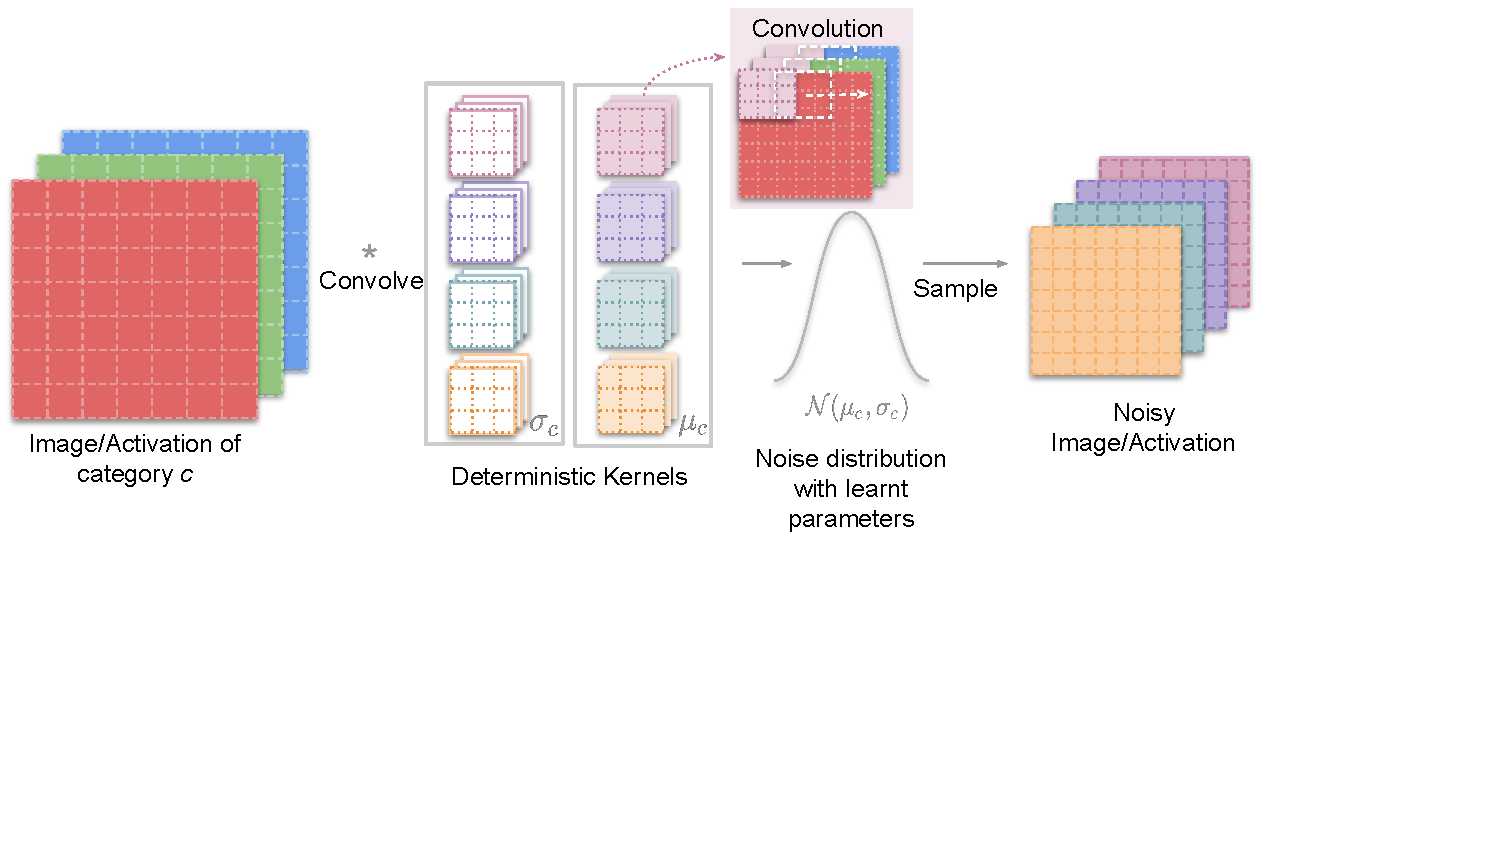
\includegraphics[width=\textwidth, trim={0 5cm 2.5cm 0}, clip]{Conditional noise layer.pdf}
    \caption{Stochastic conditional convolutional layer with learnt kernels $\mu_c$ and $\sigma_c$. The conditional probability distributions $\mathcal{N}(\mu_c, \sigma_c)$ are conditioned on the image category or label $c$.}
    \label{fig:condconv}
\end{figure}

\subsubsection{(Our Innovation) Stochastic conditional convolutional layers}
\label{sec:stochasticcondconv}
To introduce stochasticity, the output activations ($h_{k_c}$ in Eq.~\eqref{eq:condconv}), obtained as a result of the convolution operation between input $x$ and kernels $k_c$, acts as parameters of a probability distribution. 
Any probability distribution is applicable according to the use case including (but not limited to) gaussian, binomial and multinomial distributions.  
Fig.~\ref{fig:condconv} shows the mechanism where the kernels convolve over an input to produce the parameters of a gaussian distribution, mean ($\mu_c$) and standard deviation ($\sigma_c$), conditioned on the image category $c$. Instead of following the usual practice of using $h_{k_c}$ in Eq.~\eqref{eq:condconv} directly as inputs to the next layers, we sample from the parameterized probabibility distribution and use this sample as an input to the next layer. This is elaborated in Sec.~\ref{sec:training_inf}.

\subsection{Stochastic Conditional Fully Connected Layers}
We discuss stochastic conditional fully connected layers (Sec.~\ref{sec:stochasticcondfc}) by first laying the ground for fully connected layers (Sec.~\ref{sec:fc}) and conditional fully connected layers (Sec.~\ref{sec:condfc}).

\subsubsection{Fully Connected Layers} 
\label{sec:fc}
A fully connected layer performs the inner-product between the input activation vector ($x$) and the trainable parameter vector $W$.
This is represented by Eq.~\eqref{eq:linear}. The vector $h$ represents the output activation that propagates forward.
\begin{equation}
h=W \cdot x
    \label{eq:linear}
\end{equation}

\subsubsection{Conditional Fully Connected Layers}
\label{sec:condfc}
It is often useful to learn weights $W_c$ specific to the category of objects given in the training dataset. In other words, fully connected layers can be conditioned on the category of object. This is shown in Eq.~\eqref{eq:condlinear}, where $W_c$ represents the weights specific to the category $c$ in the training dataset.

\begin{equation}
h_c=W_c \cdot x
    \label{eq:condlinear}
\end{equation}

\subsubsection{(Our Innovation) Stochastic Conditional Fully Connected Layers}
\label{sec:stochasticcondfc}
To introduce stochasticity, the output activations ($h_c$ in Eq.~\eqref{eq:condlinear}) obtained as a result of the inner product between the input $x$ and weights $W_c$ acts as parameters of a probability distribution. 
Any probability distribution is applicable according to the use case including (but not limited to) gaussian, binomial and multinomial distributions.  
Instead of using $W_{c}$ in Eq.~\eqref{eq:condlinear} directly as inputs to the next layers, we sample from the probabibility distribution and use the sample as an input to the next layer. This is elaborated in Sec.~\ref{sec:training_inf}.


\section{Applications}
\label{sec:app}
Stochastic conditional layers are useful for multi-class classification, multi-object detection, semantic and instance segmentation, multi-object tracking, and many more applications. We elaborate multi-class image classification (\ref{sec:classification}) and multi-object detection (\ref{sec:detection}) applications in this section. We also demonstrate how stochastic conditional layers can be used in the context of federated learning (\ref{sec:fed}) for multi-class image classification. Note that stochastic conditional layers are applicable to other use-cases.

\subsection{Multi-Class Image Classification}
\label{sec:classification}
\begin{figure}[h!]
    \centering
    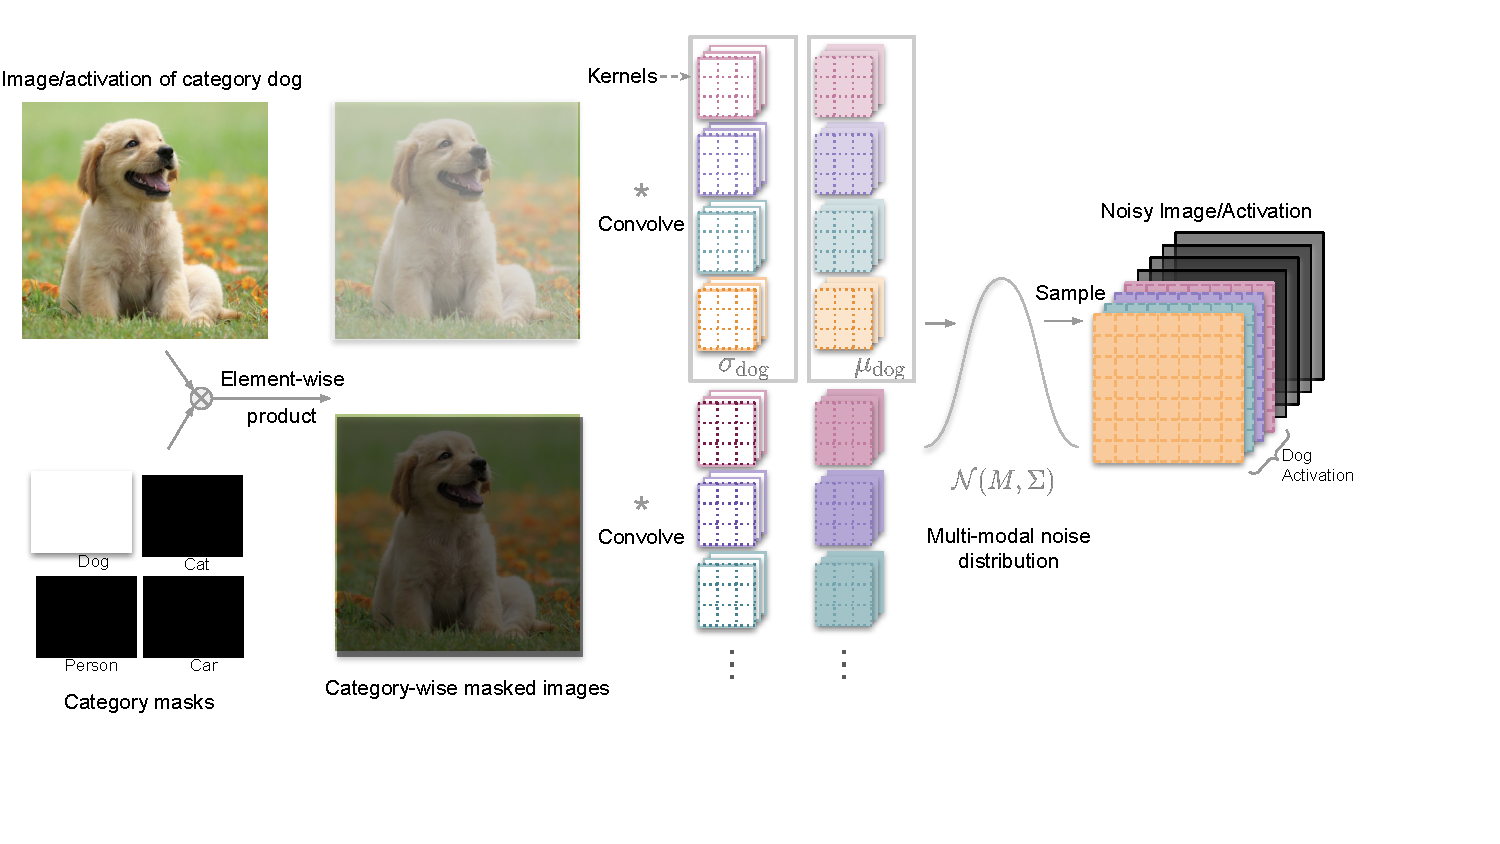
\includegraphics[width=\textwidth, trim={0cm 2cm 2.4cm 0.5cm}, clip]{Classification Conditional noise layer.pdf}
    \caption{Stochastic conditional convolutional layer for multi-class classification. The multi-modal conditional probability distribution $\mathcal{N}(M, \Sigma)$, where $M=\{\mu_c\}$ and $\Sigma=\{\sigma_c\}$) is used to sample the output activation. $\mu_c$ and $\sigma_c$ are conditioned on the image category or label $c$ ($c=$ dog in this case). During training, the tensor $\pi_\mathrm{dog}$ in the hard selection layer is $1$. All other tensors in the hard selection layer are $0$. Learnt soft selection layer is used during inference.}
    \label{fig:classification}
\end{figure}
Multi-class image classification is the task of categorizing an image into one class or category, when the training dataset contains multiple categories. We can obfuscate a given image using different embodiments of stochastic conditional layers as described in Sec.~\ref{sec:embodiments}. 
The training and inference procedures of stochastic layers in the context of multi-class image classification are described in Sec.~\ref{sec:training_inf}.

\subsubsection{(Our Innovation) Selection Layer}
To use stochastic conditional layers during inference, when the category of images (labels) are not known, we develop the idea of selection layers as shown in Fig.~\ref{fig:classification}. Selection layers are used to combine the stochastic conditional layer that are designated for different labels. Each selection layer consists of $C$ tensors, if there are $C$ total categories in the training dataset.
In one incarnation, each of the $C$ tensors is element-wise multiplied with the input $x$ before being convolved with all the convolutional kernels. In another incarnation, each of the $C$ tensors is element-wise multiplied with the output obtained when the input $x$ is convolved with all the convolutional kernels. We elaborate the use of selection layer below, with respect to the first incarnation described above.

\noindent \textbf{ Hard Selection Layer:}
During training of stochastic layers, the label for each image $x$ is known. We can use a variant of the selection layer, called hard selection layer, where the $C$ tensors have fixed pixel values $0$ or $1$ depending on the image category. The pixel values are $1$ if the image matches the certain category. Otherwise, the pixel values are $0$. This ensures that the given image of category $c$, only passes through kernels $\mu_c$ and $\sigma_c$, and no other sets of kernels, when $x$ is element-wise multiplied with each tensor in the selection layer. The hard selection layer is shown in Fig.~\ref{fig:classification}. 

\noindent \textbf{Soft Selection Layer:} When the stochastic layers are fully trained using the hard selection layer described above, we make the selection layer trainable, and remove the constraint of $0$ or $1$ on the pixel values. The selection layer can have real pixel values between $0$ and $1$ and is called the soft selection layer. Each pixel value represents a probability that the particular region in the input is of interest for a category $c$. Freezing the trained stochastic layers, we train the parameters of the soft selection layer. This soft selection layer is used to combine the stochastic conditional layer during inference tasks, when the image category is not known.

\subsection{Multi-Object Detection}
\label{sec:detection}
\begin{figure}[h!]
    \centering
    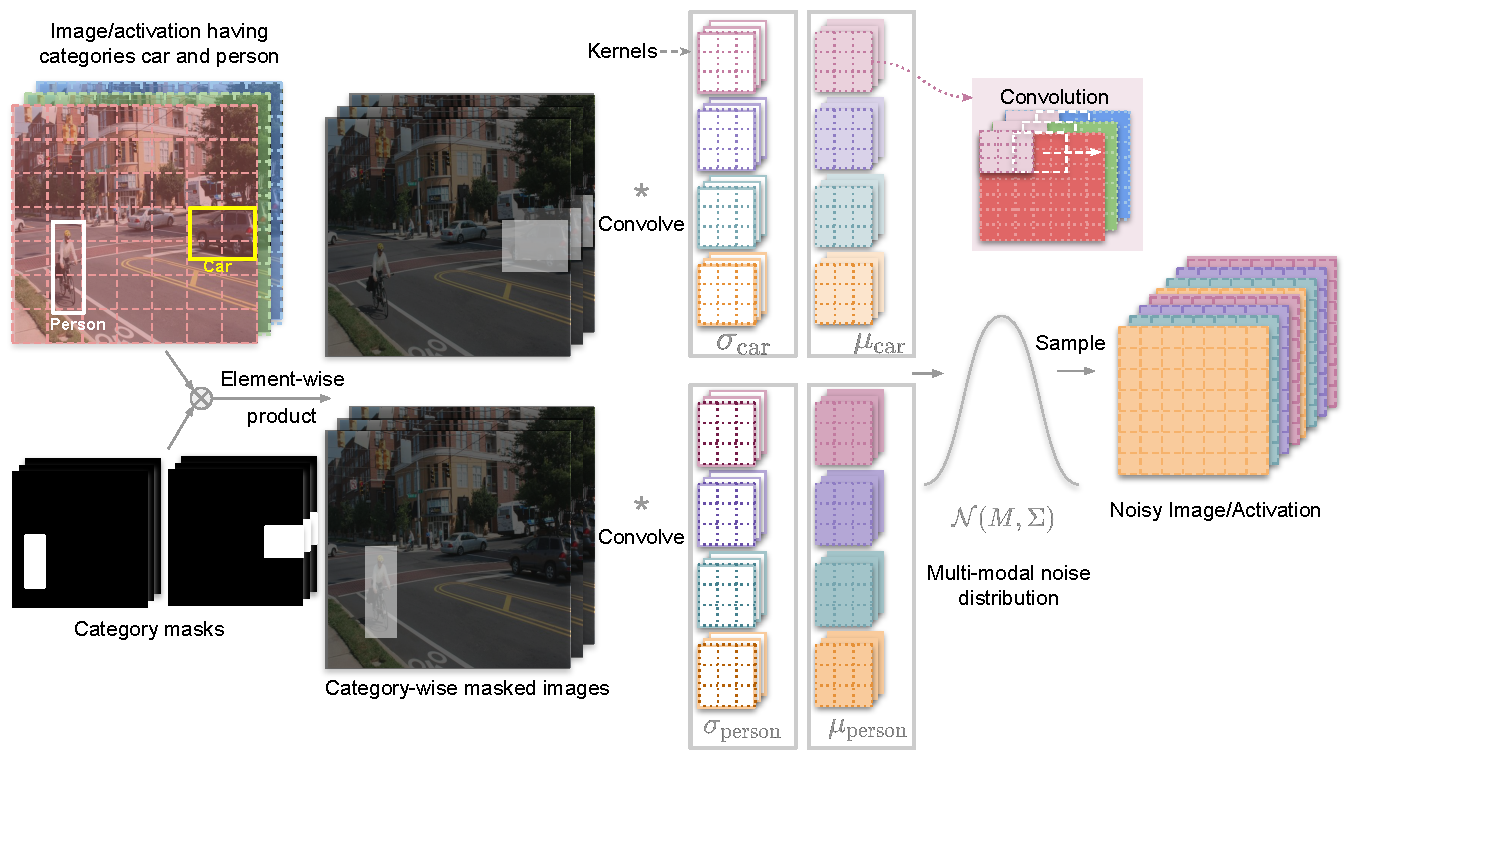
\includegraphics[width=\textwidth, trim={0cm 1.6cm 2.7cm 0cm}, clip]{Detection Conditional noise layer.pdf}
    \caption{Stochastic conditional convolutional layer for multi-object detection. The multi-modal conditional probability distribution $\mathcal{N}(M, \Sigma)$, where $M=\{\mu_c\}$ and $\Sigma=\{\sigma_c\}$) is used to sample the output activation. $\mu_c$ and $\sigma_c$ are conditioned on the image category or label $c$ ($c$ is person or car in this case). The tensor $\pi_c$ in the hard selection layer have pixel values $0$ or $1$ during training, depending on the region of interest of category $c$. Trained soft selection layer is used during inference.}
    \label{fig:det}
\end{figure}

\begin{figure}[h!]
    \centering
    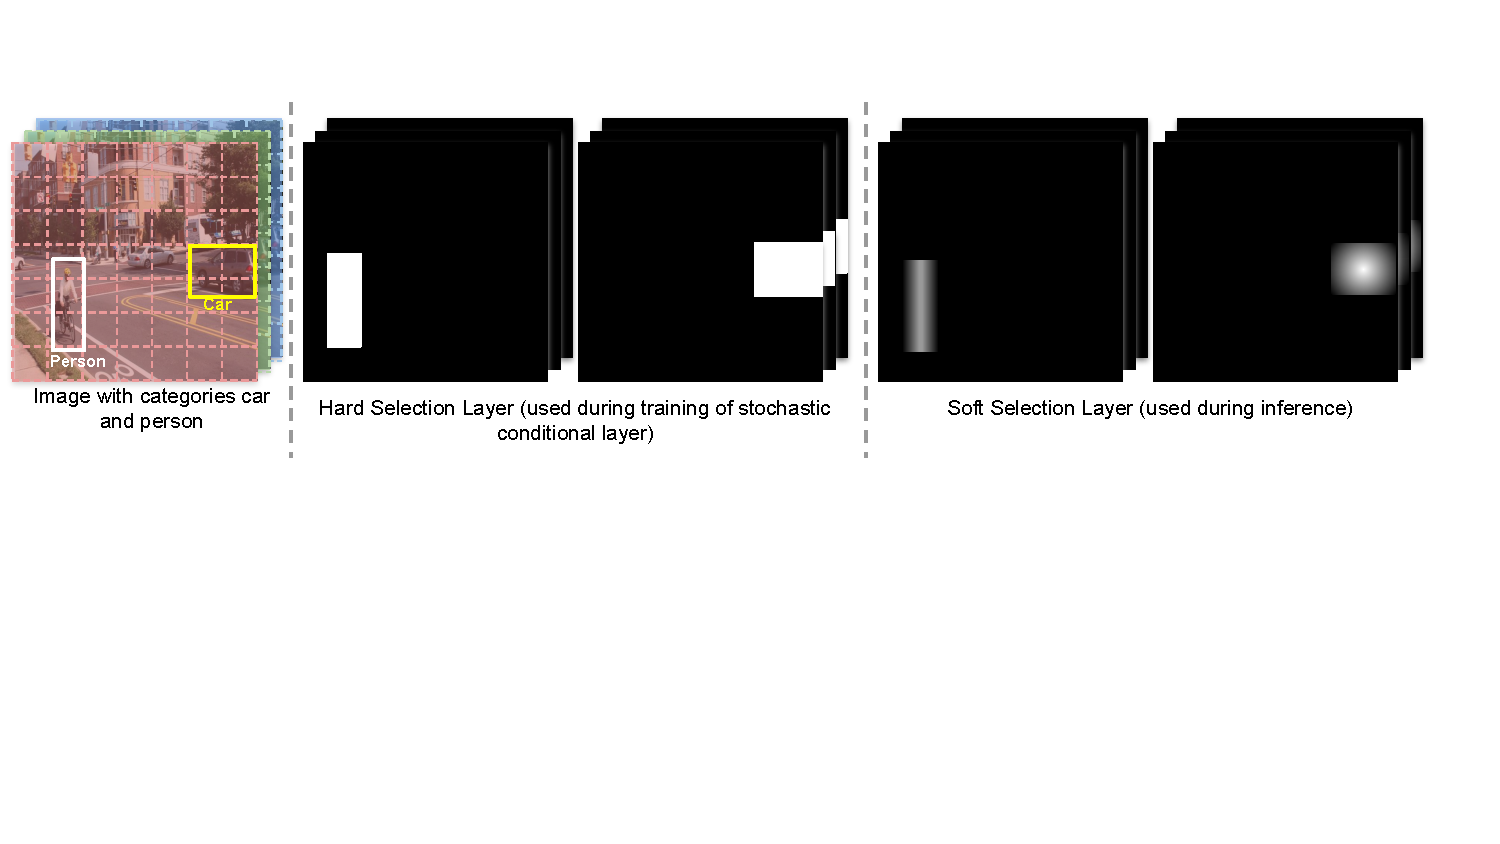
\includegraphics[width=\textwidth, trim={0cm 7cm 1cm 2cm}, clip]{category_masks.pdf}
    \caption{Selection layers used during training of stochastic layers and during inference. During training of stochastic layers, hard selection layer is used, where tensors have pixel values $0$ or $1$. Trained soft selection layer is used during inference, where pixel values are real and vary between $0$ and $1$, representing the  probability that the particular pixel in tensor $\pi_c$ belongs to class $c$.}
    \label{fig:category_masks_det}
\end{figure}

Multi-Object detection is the task of categorizing and localizing multiple objects, given an image. For example, objects of the categories ``person'' and ``car'' are to be detected in the input image shown in Fig.~\ref{fig:det}. We can obfuscate a given image using different embodiments of stochastic conditional layers as described in Sec.~\ref{sec:embodiments}. 
The training and inference procedures of stochastic conditional layers in the context of multi-object detection is similar to Sec.~\ref{sec:training_inf}.

\subsubsection{(Our Innovation) Selection Layer}
To use stochastic conditional layers during inference, when the category of objects in an images (labels) are not known, we develop the idea of selection layers as shown in Fig.~\ref{fig:det}. Selection layers are used to combine the stochastic conditional layer that are designated for different labels. Each selection layer consists of $C$ tensors of the same size as input $x$, if there are $C$ total categories in the training dataset.
Each of the $C$ tensors is element-wise multiplied with the input $x$ before being convolved with all the convolutional kernels. We elaborate the use of selection layer below.

\noindent \textbf{Hard Selection Layer:}
During training of stochastic layers, the label for each object in the image $x$ is known. We can use a variant of the selection layer, called hard selection layer, where the $C$ tensors have fixed pixel values $0$ or $1$ depending on the object category of the image. The value is $1$ if the object matches the certain category. Otherwise, the value is $0$. This ensures that the given object of category $c$, only passes through kernels $\mu_c$ and $\sigma_c$, and no other sets of kernels, when the input image $x$ is element-wise multiplied with each tensor in the selection layer. The hard selection layer during the training of the stochastic conditional kernels is shown in Fig.~\ref{fig:det} and Fig.~\ref{fig:category_masks_det} (middle figure). The white pixels indicate the value of 1, and black pixels indicate the value of 0. This ensures that the regions of interests are retained when the input image $x$ is element-wise multiplied with each tensor in the selection layer.

\noindent \textbf{Soft Selection Layer:} When the stochastic layers are fully trained using the hard selection layer, we make the selection layer trainable, and remove the constraint on the selection layer to have fixed pixel values $0$ or $1$. The selection layer can have real pixel values between $0$ and $1$ and is called the soft selection layer. Each pixel represents a probability that the particular region is of interest for a certain category. Freezing the trained stochastic layers, we now train the parameters of the selection layer. The trained soft selection layer (Fig.~\ref{fig:category_masks_det} (right)) is used to combine the stochastic conditional layer during inference tasks, when the object categories are not known.

\subsection{Federated Learning}
\label{sec:fed}
We discuss learning of the stochastic noise layer in the federated learning setting. Any task like multi-class classification, multi-object detection, etc, can be considered for this. We discuss one embodiment of the federated learning procedure on the task of multi-class classification. Other embodiments follow similar procedure. Other embodiments, nonetheless, are not limited to federated learning.

\begin{enumerate}
    \item We train a given neural network on 5\% of the training dataset, instead of the entire dataset. Let us call this trained neural network NN-5.
    \item We use NN-5 to train the stochastic conditional layer described earlier. We call this stochastic layer SL-5.
    \item We already have 5\% of the pure dataset. We obfuscate the rest 95\% of the training data using SL-5 and regulariztion technique described in Sec.~\ref{sec:reg}.  
    \item We then resume training of NN-5 on this 5\% pure and 95\% noisy dataset (obtained from the previous step). Let's call this trained neural network NN’-5.
    \item We gradually make more training data available (10\%, 15\%, etc) and iterate over steps 1,2,and 3, until the desired accuracy is reached.
\end{enumerate}

\subsubsection{(Our Innovation) Regularization}
\label{sec:reg}
In step 3 of the federated learning embodiment described above, we obfuscate 95\% of the training data using a stochastic layer training on only 5\% of the pure training dataset (SL-5). Note that this noisy data coming from the stochastic layer will be highly biased towards the small ratio of the data SL-5 was trained on. To reduce this bias, we propose a regularization step where we randomly screen parts of the noisy data at every iteration of the training, so that the screened parts aren't visible to the neural network. 

\section{Training and Inference of Stochastic Conditional Layers}
\label{sec:training_inf}
 
In this section, we elaborate the training and inference procedures for the stochastic conditional layers, considering the convolutional incarnation and by assuming a gaussian distribution for the output activations for the task of multi-class classification. Other physical incarnations, types of distributions and applications will have similar procedures. We describe several applications in Sec.~\ref{sec:app}


\subsection{Training} 
We describe training as a two step procedure. In the first step, we learn the weights of the stochastic conditional layer. In the next step, we learn the weights of the soft selection layers (described in Sec.~\ref{sec:classification}) that are necessary during inference. The steps are described below. Note that the training pipeline can be different depending on applications. For example, step 2 can be omitted if the user is aware of the class labels. Hard Selection layers can be used in that case (Sec.~\ref{sec:classification}). Fig.~\ref{fig:classification} describes a forward pass during the training procedure for the task of multi-class image classification.

\subsubsection{Training of Stochastic Conditional Layer}
Prior to training, two sets of kernels ($k_{\mu_c}$ and $k_{\sigma_c}$) are initialized for the two parameters, in a gaussian distrubution, mean ($\mu_c$) and standard deviation ($\sigma_c$) respectively, conditioned on each category $c$ out of the total $C$ categories in the training dataset. During the forward pass, the kernels $k_{\mu_c}$ and $k_{\sigma_c}$ perform convolution operation on the input activation $x$, if $x$ belongs to the category $c$. In other words, $x$ is first multiplied with all the $C$ tensors in the hard selection layer, $\pi_c$, which have pixel values $1$ if $x$ belongs to category $c$, and $0$ if $x$ belongs to any other category. This modified input is then passed through the stochastic conditional layer. The output activation maps ($\mu_c$ and $\sigma_c$) are obtained from the respective set of kernels according to Eq.~\eqref{eq:mu_c} and Eq.~\eqref{eq:sigma_c}. $\mu_c$ and $\sigma_c$ (mean and standard deviation) are used to define the gaussian distribution. We randomly sample an activation map  $h_c$ from this distribution according to Eq.~\eqref{eq:sample}. $h_c$ acts as an input activation for the next layers in the network. 

\begin{equation}
  \mu_c[m,n]=(x * k_{\mu_c})[m,n]=\sum_i \sum_j k_{\mu_c}[i,j]x[m+i,n+j]
  \label{eq:mu_c}
\end{equation}
\begin{equation}
  \sigma_c[m,n]=(x * k_{\sigma_c})[m,n]=\sum_i \sum_j k_{\sigma_c}[i,j]x[m+i,n+j]
  \label{eq:sigma_c}
\end{equation}

\begin{align}
  h_\mathrm{c} \sim \mathcal{N}(\mu_c,\sigma_c) \notag\\
  \Rightarrow h_c=\mu_c + \sigma_c.\epsilon;\; \epsilon \sim \mathcal{N}(0,1)
  \label{eq:sample}
\end{align}

The kernels are trained in a similar manner as standard convolutional neural networks. The parameters of the gaussian distribution for each category $\mu_c$ and $\sigma_c$ (Eq.~\eqref{eq:mu_c} and Eq.~\eqref{eq:sigma_c}), obtained in the forward pass, are differentiable with respect to the kernels $k_{\mu_c}$ and $k_{\sigma_c}$ respectively. $h_c$ is differentiable with respect to $\mu_c$ and $\sigma_c$. Gradients of the output activation $h_c$ can be obtained with respect to the kernels  $k_{\mu_c}$ and $k_{\sigma_c}$. The kernels are trainable using the aforementioned gradients through back-propagation and gradient descent. 

\subsubsection{Training of Soft Selection Layer}
The selection layer can directly be applied to the input $x$. As other embodiments, the selection layer can also be applied after the stochastic layers, or anywhere in the neural network. We describe the training procedure considering that the selection layer is applied directly on the input.

The input $x$ is multiplied with trainable tensor of the soft selection layer $\pi_c$ whose values are real and vary between $0$ and $1$, representing the probability of the image belonging to a certain category $c$. If there are $C$ categories in the dataset, there are $C$ tensors in the soft selection layer to be trained. $\pi=\{\pi_c\}$ represents all the tensors concatenated together. The modified input ($x \bigotimes \pi$) undergoes forward pass. The activations at every step are differentiable with respect to the tensors in the soft selection layer and hence backpropagation and gradient descent are directly applicable to train the soft selection layer.
The step involving training of the soft selection layer can be omitted if the user is aware of the input category when the input is passed through the stochastic conditional layer. In that case, we can use the hard selection layer, where $\pi_c=1$ if $x$ belongs to category $c$, otherwise $\pi_c=0$. 

\subsection{Inference}
The kernels $k_{\mu_c}$ and $k_{\mu_c}$ and tensors in the soft selection layer, $\pi_c$, are trained according to the previous sub-section. A forward pass is performed using the category masks and trained kernels to produce the a parameterized probability distribution, from which the output activation map $h_c$ is sampled. The output activation map acts as an input activation for the next layer in the neural network. 

\section{Related Work}
Previous works attempted to ensure that the accuracy of the deep networks trained on very little carefully crafted or chosen training data, remain similar to the accuracy of the deep networks trained on full training datasets. Some of these attempts are described next.

\noindent \textbf{Dataset distillation:} Wang et al.~\cite{datasetdistillation} learned a small number of data points that do not need to come from the correct data distribution.  A model trained on these synthetic data points approximate a model trained on the original data well.

\noindent \textbf{Active learning:} Active learning \cite{al1,al2,al3,al4} attempts to maximize the performance of models while annotating very little training data. The deep model is first trained using a small set of annotated training data.  The model queries a user to label selected unlabelled samples for which the model had the lowest prediction confidence. 

\section{Embodiments of Stochastic Conditional Layers}
\label{sec:embodiments}
We consider a neural network $N$, input $x$, a stochastic conditional layer $S_L$, and $n$ additional regular layers $L_{i\text{\{$i=0$ to $n$\}}}$. In the normal state of using $N$, the input is applied to $N$ without the involvement of $S_L$ or $L_i$. We propose a few embodiments as described below.
\begin{enumerate}
    \item In one embodiment, we propose this new arrangement as shown. $x \rightarrow L_{i\text{\{$i=0$ to $n$\}}} \rightarrow S_L \rightarrow N$.
    \item In another embodiment, we break $N$ into two parts $N_1$ and $N_2$, where $N$ is equivalent to $N_1$,$N_2$ back to back. Let $O_1$ be the output of applying $N_1$ to $x$, i.e., $O_1 = x \rightarrow N_1$. Let $O_2$ be the output of applying $L_{i\text{\{$i=0$ to $n$\}}}$ to $x$, i.e., $O_2 = x \rightarrow L_{i\text{\{$i=0$ to $n$\}}}$. Then, we merge $O_1$ and $O_2$ and pass the merged results through $S_L$. We then pass the resulting activations through $N_2$.
    \item In another embodiment, we apply $S_L$ to $O_2$, then merge the results with $O_1$, and then pass the result through $N_2$.
    
\end{enumerate}

{\small
\bibliographystyle{ieee_fullname}
\bibliography{egbib}
}

\end{document}
